\label{sec::outlier}

For performance logs generated from large numbers of processors, it is
often difficult to view in detail the behavior of poorly behaved
processors. This view attempts to present information similar to usage
profile but only for processors whose behavior is ``extreme''.

\begin{figure}[htb]
\center
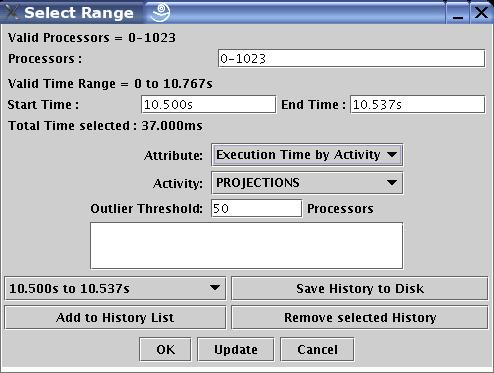
\includegraphics[width=4.0in]{fig/outlier_dialog}
\caption{Outlier Analysis Selection Dialog}
\label{outlier dialog}
\end{figure}

``Extreme'' processors are identified through the application of
heuristics specific to the attribute that analysts wish to study
applied to a specific activity type. You can specify the number of
``extreme'' processors are to be picked out by \projections{} by
filling the appropriate number in the field ``Outlier Threshold''. The
default is to pick 10\% of the total number of processors up to a cap
of 20. As an example, an analyst may wish to find ``extreme''
processors with respect to the idle time of normal \charmpp{} trace
events.

Figure \ref{outlier dialog} shows the choices available to this
tool. Specific to this view are two pull-down menus: {\em Attribute}
and {\em Activity}.

There are four {\em Activity} options:
\begin{enumerate}
\item The {\em Projections} activity type refer to the entry methods 
executed by the \charmpp{} runtime system.
\item The {\em User Events} activity type refer to records of events
as captured through {\tt traceUserEvent}-type calls described in
section \ref{sec::user events}.
\end{enumerate}

There are four {\em Attribute} options:
\begin{enumerate}
\item {\em Execution time by Activity} tells the tool to apply heuristics
based on the execution time of each instance of an activity occurring
within the specified time range.
\item {\em Idle time} tells the tool to apply a simple sort over all
processors on the least total idle time recorded. This will work only for
the {\em Projections} activity type.
\item {\em Msgs sent by Activity} tells the tool to apply heuristics
based on the number of messages sent over each instance of an
activity occurring within the specified time range. This option is
currently not implemented but is expected to work over all activity
types.
\item {\em Bytes sent by Activity} tells the tool to apply heuristics
based on the size (in bytes) of messages sent over each instance of an
activity occurring within the specified time range. This option is
currently not implemented but is expected to work over all activity
types.
\end{enumerate}

\begin{figure}[htb]
\center
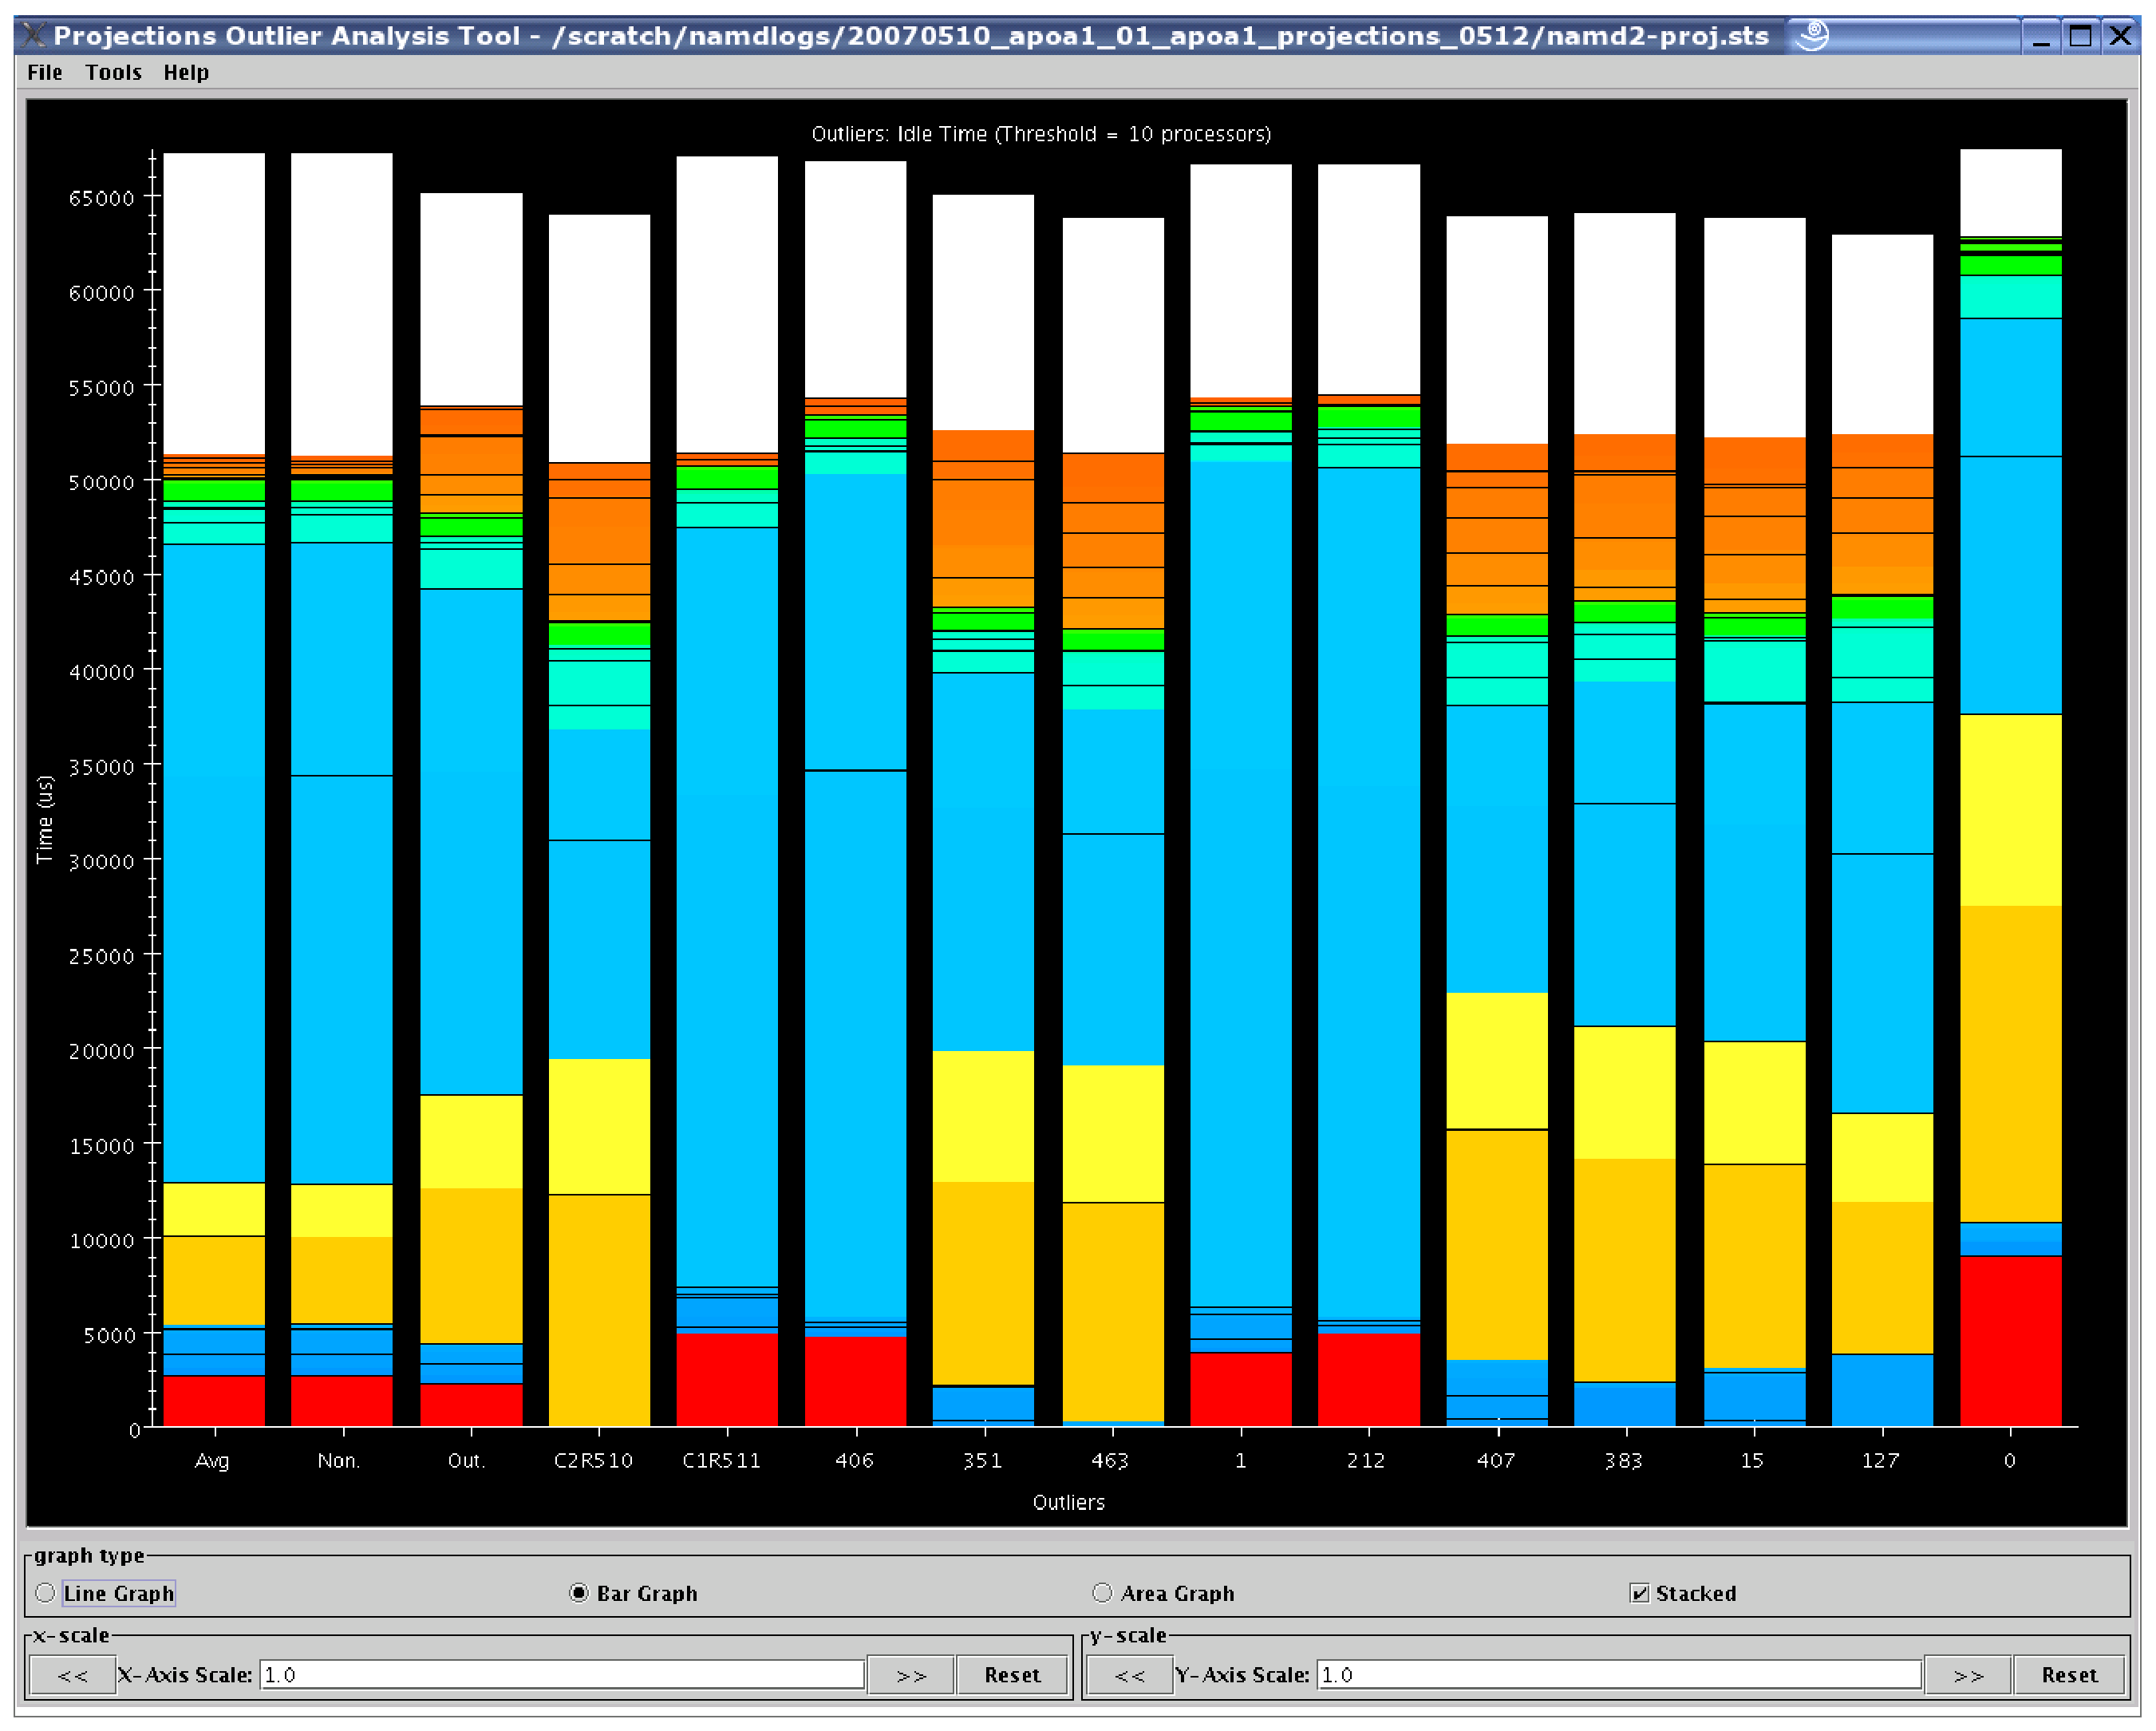
\includegraphics[width=4.0in]{fig/apoa1_512_outlierWithClusters}
\caption{Outlier Analysis View}
\label{outlier view}
\end{figure}

At the same time, a k-means clustering algorithm is applied to the
data to help identify processors with exemplar behavior that is
representative of each cluster (or equivalence class) identified by
the algorithm. You can control the value of k by filling in the
appropriate number in the field ``Number of Clusters''. The default
value is 5.

The result of applying the required heuristics to the appropriate {\em
attribute} and {\em activity} types results in a chart similar to
figure \ref{outlier view}. This is essentially a usage profile that
shows, over the user's selected time range, from left to right:

\begin{itemize}
\item A bar representing the global average of execution time of each
activity over all processors.
\item A bar representing the average activity profile of all
non-outlier (or non-extreme) processors.
\item A bar representing the average activity profile of all outlier
(or extreme) processors identified by the heuristics.
\item One bar representing the activity profile of the representative
processor from each cluster of processors identified by the application
of the k-means clustering algorithm.
\item One bar representing the activity profile of each identified
outlier processor, sorted in order of significance (rightmost processor
bar is the most significant).
\end{itemize}

The tool helps the user reduce the number of processor bars that must
be visually examined in order to identify candidates for more detailed
study. To further the cause of this goal, if the analyst has the {\em
timeline} view (see section \ref{sec::timeline view}) open, a
mouse-click on any of the processor activity profile bars (except for
group-averaged bars) will load that processor's detailed timeline
(over the time range specified in the timeline view) into the timeline
view itself.

%\begin{figure}[htb]
%\center
%\includegraphics[width=4.0in]{fig/outlier_dialogAttributes}
%\caption{Outlier Analysis Attributes available}
%\label{outlier attributes}
%\end{figure}

%\begin{figure}[htb]
%\center
%\includegraphics[width=4.0in]{fig/outlier_dialogActivities}
%\caption{Outlier Analysis Activity Types available}
%\label{outlier activities}
%\end{figure}

